\documentclass[a4paper]{article}
\usepackage[utf8]{inputenc}
\usepackage[slovene]{babel}
\usepackage{graphicx}
\usepackage{hyperref}
\usepackage[nottoc]{tocbibind}
\usepackage{caption}
\usepackage{subcaption}
\usepackage{amsmath}
\usepackage{ dsfont }
\usepackage{siunitx}
\usepackage{multimedia}
\usepackage[table,xcdraw]{xcolor}
\usepackage{float}
\setlength\parindent{0pt}

\newcommand{\ddd}{\mathrm{d}}
\newcommand\myworries[1]{\textcolor{red}{#1}}
\newcommand{\Dd}[3][{}]{\frac{\ddd^{#1} #2}{\ddd #3^{#1}}}

\begin{document}
\begin{titlepage}
    \begin{center}
        
\includegraphics[]{logo.png}
        \vspace*{3cm}
        
        \Huge
        \textbf{Modeli kemijskih reakcij}
        
        \vspace{0.5cm}
        \large
        5. naloga pri Modelski Analizi 1

        \vspace{4.5cm}
        
        \textbf{Avtor:} Marko Urbanč (28232019)\ \\
        \textbf{Predavatelj:} prof. dr. Simon Širca\ \\
        \textbf{Asistent:} doc. dr. Miha Mihovilovič\ \\
        
        \vspace{2.8cm}
        
        \large
        8.11.2023
    \end{center}
\end{titlepage}
\tableofcontents
\newpage
\section{Uvod}
Čeprav smo fiziki in smo na študiju fizike, ne moremo zanikati, da je tudi kemija pomembna veda. A izkaže se, da 
ni vedno najbolj ugodno narediti prav vsak eksperiment v živo. Zato se je razvil računalniški pristop,
ki nam omogoča, da lahko simuliramo različne kemijske reakcije. Pravzaprav je pristop praktično analogen
prejšnji nalogi o populacijskih modelih. No vsaj ko naredimo ustrezne približke. V resnici, če bi hoteli brez kompromisa
modelirati kemijske procese, bi nas to drago stalo. To mislim dobesedno, ker če bi reševali t.i. \textbf{Chemical master
equation} bi dobili sistem ODE s toliko komponent, kolikor je možnih stanj sistema. To pa je, če želimo simulirati nek
makroskopski proces, zelo veliko. Zato se bomo v tej nalogi omejili na reševanje \textbf{Reaction rate} enačb, ki so
približek prej omenjenih enačb. V tej nalogi bomo spoznali modeliranje kemijskih procesov na podlagi treh primerov.\\

\subsection{Binarna reakcija}
Za prvi primer si poglejmo primer binarne reakcije. Kemijske procese lahko opišemo kot:

\begin{gather}
    A + A \overset{p}{\underset{q}{\rightleftharpoons}} A + A^*\>,\\
    A^* \overset{r}{\rightarrow} B + C\>.
\end{gather}

Rate enačbe v brezdimenzijski obliki za proces dobimo tako, da vse koncentracije normiramo
z začetno koncentracijo snovi $A$ $[A](0)$. S tem bomo lahko uvedli še nove parametre. Takole:

\begin{gather}
    \dot{a} = \frac{1}{2} kaa^* - a^2 + \frac{1}{2}a^2\>,\\
    \dot{a^*} = \frac{1}{2}a^2 - \frac{1}{2} kaa^* - ska^*\>,\\
    \dot{b} = \frac{1}{2} ska^*\>,\\
    \dot{c} = \frac{1}{2} ska^*\>.
\end{gather}

kjer je $k = \frac{p}{q}$ in $s = \frac{r}{q[A](0)}$. Odvod pa je zdaj po $d\tau = p[A](0)\>dt$. Lahko
predpostavimo, da v ravnovesnem stanju velja $\dot{a^*} = 0$, kar nam omogoči, da izrazimo $a^*$ in s tem 
dobimo nov set enačb:

\begin{gather}
    \dot{a} = \frac{a^3}{4k(s + a/2)} - a^2\>,\\
    \dot{a^*} = 0\>,\\
    \dot{b} = \frac{sa^2}{4(s + a/2)}\>,\\
    \dot{c} = \frac{sa^2}{4(s + a/2)}\>.
\end{gather}

\subsection{Sinteza vodikovega bromida}
Za drugi primer pogledamo primer sinteze vodikovega bromida. Sinteza je sestavljena iz več stopnj. Te lahko
zapišemo kot:

\begin{gather}
    \mathrm{Br}_2 \overset{p}{\underset{q}{\rightleftharpoons}} 2\mathrm{Br}\>,\\
    \mathrm{Br} + \mathrm{H}_2 \overset{r}{\underset{s}{\rightleftharpoons}} \mathrm{HBr} + \mathrm{H}\>,\\
    \mathrm{H} + \mathrm{Br}_2 \overset{t}{\rightarrow} \mathrm{HBr} + \mathrm{Br}\>.
\end{gather}

To lahko z sistemom ODE opišemo kot prej takole:

\begin{gather}
    \dot{u} = sxy - ruz\>,\\
    \dot{v} = qz^2 - pv - \frac{1}{2}tvy\>,\\
    \dot{x} = \frac{1}{2}tvy - \frac{1}{2}sxy + \frac{1}{2}ruz\>,\\
    \dot{y} = \frac{1}{2}ruz - \frac{1}{2}sxy + \frac{1}{2}tvy\>,\\
    \dot{z} = \frac{1}{2}tvy + pv - qz^2\>,
\end{gather}

kjer je $u = [\mathrm{H}_2]$, $v = [\mathrm{Br}_2]$, $x = [\mathrm{HBr}]$, $y = [\mathrm{H}]$ in $z = [\mathrm{Br}]$.
Tudi ta sistem lahko zapišemo v približku stacionarnega stanja, kjer velja $\dot{y} = 0$ in dobimo:

\begin{gather}
    \dot{u} = -\frac{1}{2}tvy\>,\\
    \dot{v} = qz^2 - pv - \frac{1}{2}tvy\>,\\
    \dot{x} = tvy\>,\\
    \dot{y} = 0\>,\\
    \dot{z} = \frac{1}{2}tvy + pv - qz^2\>.
\end{gather}

Na predavanjih je profesor omenil še možnost stacionarnega stanja za $\dot{z} = 0$, ampak meni ni uspelo
uspešno pognati reakcije v tem primeru.\\

\subsection{Kemijska ura}
Za konec pa še bolj zabaven primer, kemijska ura. Princip je, da imamo dve reakciji, ki se odvijata vzporedno.
Prva reakcija je hitra, druga pa počasna. Ko se prva reakcija konča, se začne druga in s tem se spremeni barva
raztopine. Pravzaprav imamo dve reakciji za vsako od barv, torej dve hitri in dve počasni. To lahko zapišemo kot:

\begin{gather}
    \mathrm{S}\mathrm{O}_8^{2-} + \mathrm{I}^- \overset{p_\mathrm{slow}}{\longrightarrow} \mathrm{I}\mathrm{S}_2\mathrm{O}_8^{3-}\>,\\
    2\mathrm{S}_2\mathrm{O}_3^{2-} + \mathrm{I}_2 \overset{p_\mathrm{fast}}{\longrightarrow} \mathrm{S}_4\mathrm{O}_6^{2-} + 2\mathrm{I}^-\>,\\
    \mathrm{S}_{2}\mathrm{O}_3^{2-} + \mathrm{I_2} \overset{q_\mathrm{slow}}{\longrightarrow} \mathrm{I}\mathrm{S}_2\mathrm{O}_3^{-} + \mathrm{I}^-\>,\\
    \mathrm{I}\mathrm{S}_2\mathrm{O}_3^{-} + \mathrm{S}_2\mathrm{O}_3^{2-} \overset{q_\mathrm{fast}}{\longrightarrow} \mathrm{S}_4\mathrm{O}_6^{2-} + \mathrm{I}^-\>.
\end{gather}

To sem modeliral kar po isti metodi kot prej. Označil sem $u = [\mathrm{S}_2\mathrm{O}_8^{2-}]$,
$v = [\mathrm{I}\mathrm{S}_2\mathrm{O}_8^{3'}]$, $w = [\mathrm{S}\mathrm{O}_4^{2-}]$,
$x = [\mathrm{S}_2\mathrm{O}_3^{2-}]$, $y = [\mathrm{I}\mathrm{S}_2\mathrm{O}_3^{-}]$, $z = [\mathrm{S}_4\mathrm{O}_6^{2-}]$
in $m = [\mathrm{I}^-]$ ter $n = [\mathrm{I}_2]$. Dobimo 8D sistem:

\begin{gather}
    \dot{m} = - p_\mathrm{slow}mu - p_\mathrm{fast}mv + q_\mathrm{slow}xn + q_\mathrm{fast}xy\>,\\
    \dot{n} = p_\mathrm{fast}mv - q_\mathrm{slow}xn\>,\\
    \dot{u} = - p_\mathrm{slow}mu\>,\\
    \dot{v} = p_\mathrm{slow}mu - p_\mathrm{fast}mv\>,\\
    \dot{w} = p_\mathrm{fast}mv\>,\\
    \dot{x} = - q_\mathrm{slow}nx - q_\mathrm{fast}xy\>,\\
    \dot{y} = q_\mathrm{slow}nx - q_\mathrm{fast}xy\>,\\
    \dot{z} = q_\mathrm{fast}xy\>.
\end{gather}


\section{Naloga}
Naloga nas prosi, da za binarne reakcije integriramo sistem eksaktno in
v aproksikmaciji stacionarnega stanja za različne vrednosti $s$ pri čemer je 
$k=1000$. Za sintezo vodikovega bromida pa naj v približku stacionarnega stanja
določimo empirični konstanti $k$ in $m$ izrazu:

\begin{equation}
    \dot{[\mathrm{HBr}]} = \frac{k[\mathrm{H}_2][\mathrm{Br}_2^{1/2}]}{m + [\mathrm{HBr}]/[\mathrm{Br}_2]}
\end{equation}

Skicirajmo naj poteke za hitrost sinteze vodikovega bromida v odvisnosti od začetne konentracije 
$\mathrm{H}_2$ in $\mathrm{Br}_2$. Kaj se zgodi če primešamo mnogo $\mathrm{HBr}$?\\

Na koncu pa še narišimo potek koncentracij $m$, $n$ za kemijsko uro, kjer spreminjamo razmerje
hitrosti glavnih reakcij.\\

\section{Opis reševanja}
Za to nalogo se mi zdi, da sem bil nekoliko uninspired. Imel sem velike želje, ampak je žal moja 
spužva za razmišljanje imela druge načrte ter mi je začela delat probleme. Zato sem ostal še kar 
pri železni srajci in naredil isto kot pri prejšnji nalogi. \\

Za vsak primer sem naredil svoj razred, ki ima metode za integracijo in vsebuje enačbe modela. Takole
se lahko instancira razred za različne parametre zelo hitro in z enim klicem dobiš rešitev. V ta namen sem
uporabljal standardni nabor knjižnic za numerično računanje v Pythonu, t.j. \texttt{numpy} in \texttt{scipy} in
seveda \texttt{matplotlib} za risanje. Za integrator, kar je verjetno še najbolj zanimivo, sem uporabljal
\texttt{scipy.integrate.solve\_ivp} z metodo \texttt{RK45} in \texttt{LSODA}. \\

\section{Rezultati}
\subsection{Binarna reakcija}
Verjetno je najbolje, da kar začnemo z rezultati. Najprej bi rad samo pokazal, kakšna je rešitev za
binarno reakcijo. To je prikazano na sliki \ref{fig:binarna} za dva primera. Za prvi primer sem že vzel
parametre iz naloge, v drugem pa sem jih spremenil, tako da se vidi tudi nekaj dogajanja z $a^*$, ki sicer
v prvem primeru ostane konstantno na $0$.\\

\begin{figure}[H]
    \centering
    \makebox[\textwidth][c]{%
    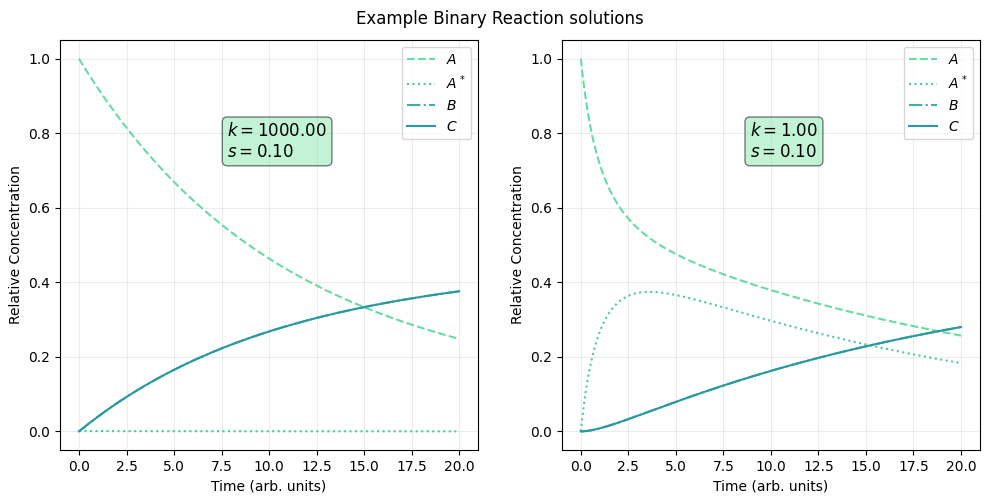
\includegraphics[width=1.2\textwidth]{../BinaryReactions/Images/basic-solution.png}
    }
    \caption{Rešitev za binarno reakcijo.}
    \label{fig:binarna}
\end{figure}

Iz te slike je precej jasno, da so parametri na levi bolj primerni za hitro sintezo $b$ in $c$, če je
naš cilj seveda. Lahko pa sta to stranska produkta, ki ju ne želimo. V tem primeru je boljši desni primer,
kjer se $a^*$ ne zadržuje na $0$, a tam je treba biti previden, ker se $a^*$ poveča nato pa spet zmanjša, 
torej bi morali v tem primeru reakcijo zaustaviti, ko je $a^*$ na vrhuncu.\\

Če si pogledamo zdaj zahtevane rešitve, dobimo sliko \ref{fig:binarna-req}. Zdelo se mi je zanimivo,
da bi za pokazal še kako se bolj zvezno spreminja vsota $b + c$, zato sem jo tudi narisal. Tu bi bilo 
smiselno potem, da sta to produkta, ki ju želimo.\\

\begin{figure}[H]
    \centering
    \makebox[\textwidth][c]{%
    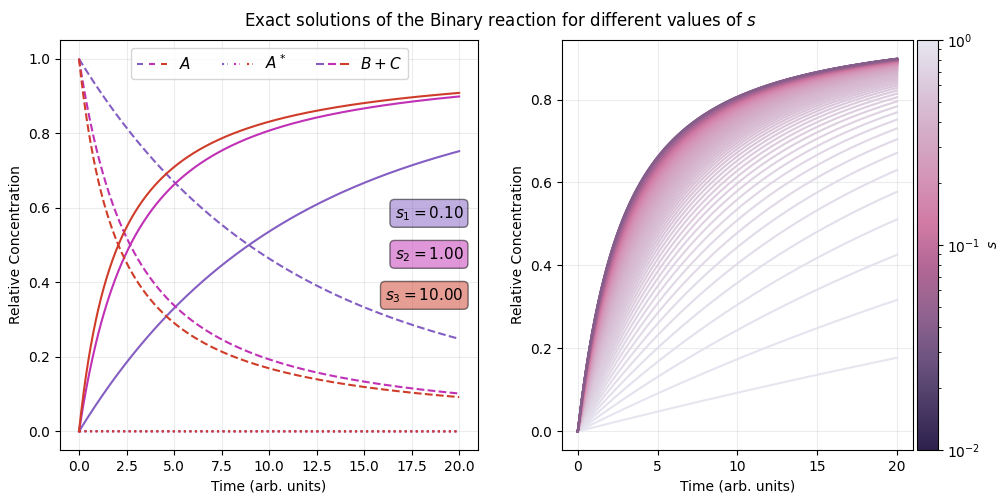
\includegraphics[width=1.2\textwidth]{../BinaryReactions/Images/exact-solution.png}
    }
    \caption{Točna rešitev.}
    \label{fig:binarna-req}
\end{figure}

Vidimo, da za majhne parametre $s$ hitrost limitira proti neki, recimo temu, kritični hitrosti. Tukaj 
sicer nisem uspel lepo narisati limitne hitrosti. Je pa to storjeno na kasnejšem primeru. Za velike parametre
pa hitrost limitira proti $0$. To je seveda pričakovano, saj parameter $s$ otežuje reakcijo iz $a^*$ v $b$ in $c$. \\

V približku ravnovesnega stanja pa sem dobil sliko \ref{fig:binarna-stac}. Tu se koncentracija zelo hitro
izravna, torej lahko z parametrom $s$ zelo dobro vplivamo na koncentracijo $b$ in $c$ v končnem stanju. To bi 
bilo koristno. če bi bila ta reakcija precursor za nek daljši proces.\\

\begin{figure}[H]
    \centering
    \makebox[\textwidth][c]{%
    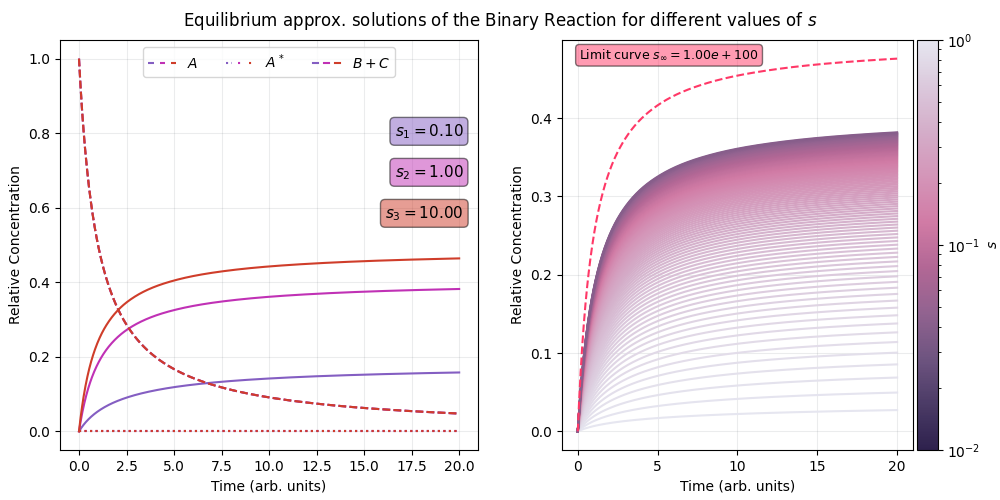
\includegraphics[width=1.2\textwidth]{../BinaryReactions/Images/equilibrium-solution.png}
    }
    \caption{Rešitev v približku ravnovesnega stanja.}
    \label{fig:binarna-stac}
\end{figure}

Tu pa sem uspel dobiti limitno krivuljo, tako da sem vzel $s = 10^{100}$ (in še velikostne rede okoli) in ugotovil,
da se družina krivulj zbere v krivulji, ki kaže proti vsoti $0.5$. Zdaj pri drugi evalvaciji mi sicer da misliti, da sem
se mogoče pri normalizaciji rešitve zmotil za faktor $2$, ker bi morala vsota koncentracij biti $1$. Ampak recimo, 
da se razume, kaj je mišljeno.\\

\subsection{Sinteza vodikovega bromida}
Spet si najprej poglejmo neko osnovno rešitev, kjer so narisane vse komponente. To je prikazano na sliki 
\ref{fig:br-basic} za dva različna primera začetnih koncentracij in hitrosti reakcij. Vektor koncentracij
je urejen tako, da je $[u, v, x, y, z]$. Vektor hitrosti reakcij pa je $[p, q, r, s, t]$.

\begin{figure}[H]
    \centering
    \makebox[\textwidth][c]{%
    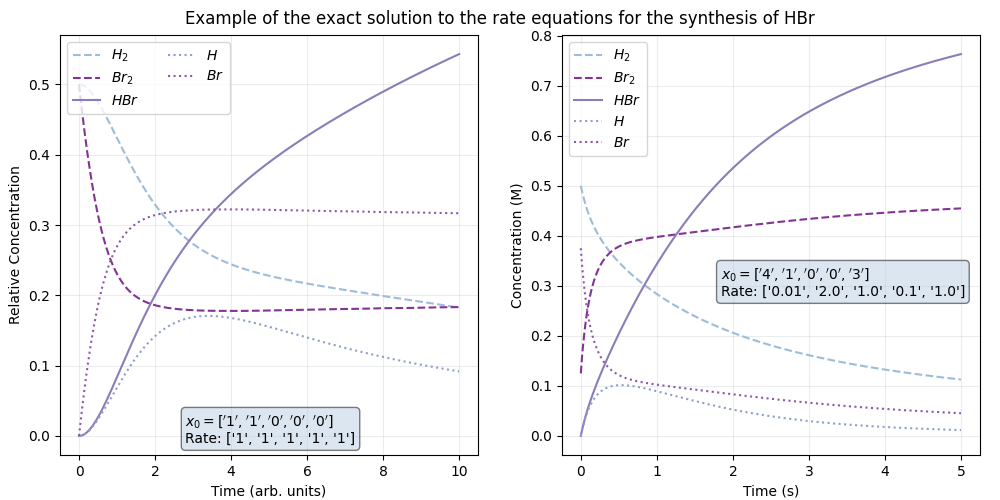
\includegraphics[width=1.2\textwidth]{../HydrogenFusion/Images/basic-solution.png}
    }
    \caption{Rešitev za sintezo vodikovega bromida.}
    \label{fig:br-basic}
\end{figure}

Vidimo, da je dogajanje tu precej bolj zanimivo kot pri binarni reakciji. Zanimivo je, kako se na levem 
primeru koncentracija $\mathrm{Br}_2$ ustali na neki vrednosti, medtem ko na desni najprej skoči in se nato 
počasi povečuje. Res je težko reči, kaj je boljše, ker je odvisno od tega, kaj želimo. Še sploh pa, nisem
kemik in ne vem, kaj je sploh koristen produkt. Če je cilj sinteza $\mathrm{HBr}$, potem je boljši desni primer,
ker se $\mathrm{HBr}$ hitreje sintetizira. \\

Model sem poskusil rešiti še v stacionarnem stanju, ampak sem dobil porazno slabe rezultate v tem smislu,
da se reakcija, kljub zadostni količini reaktantov, nikoli ni začela. Zato sem se odločil, da bom raje
določil konstanti $k$ in $m$ za eksakten model. Vseeno je na sliki \ref{fig:br-stac} na desni prikazana 
rešitev v približku stacionarnega stanja. Za primerjavo je na levi točna rešitev za iste parametre.\\

\begin{figure}[H]
    \centering
    \makebox[\textwidth][c]{%
    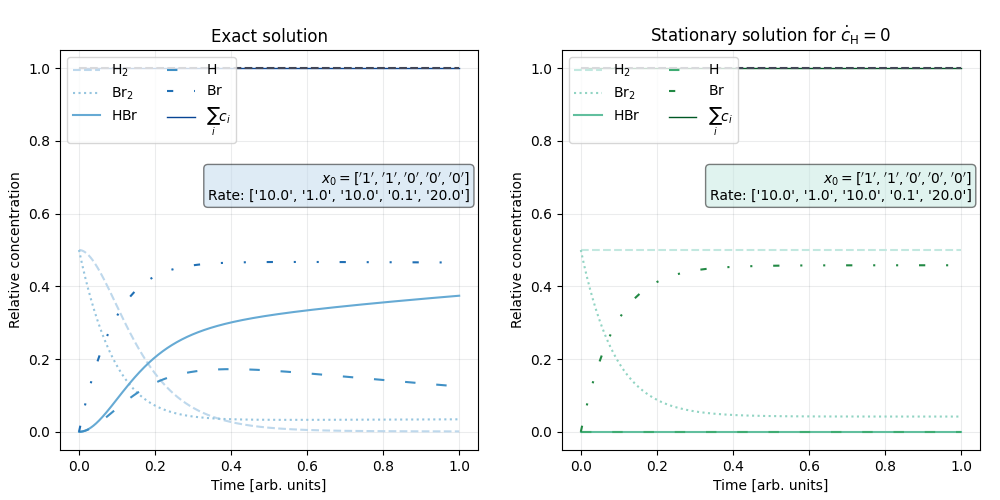
\includegraphics[width=1.2\textwidth]{../HydrogenFusion/Images/wont-start.png}
    }
    \caption{Porazna rešitev v približku ravnovesnega stanja, ki ne začne.}
    \label{fig:br-stac}
\end{figure}

Torej potem, kako najlažje določiti konstanti $k$ in $m$? Trudil sem se, da bi problem nekako lineariziral.
Že imena parametrov spominjata na kakšno premico, ampak tega nisem uspel narediti. Zato sem se na koncu odločil 
za hitro primerjavo preliminary fit metod, po katerih lahko posežemo, ko je treba za silo prilagoditi neko krivuljo.
Rezultati so prikazani na sliki \ref{fig:br-fit}.\\

\begin{figure}[H]
    \centering
    \makebox[\textwidth][c]{%
    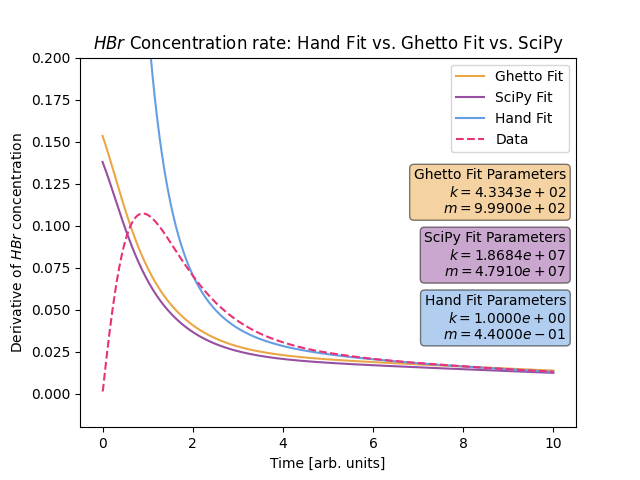
\includegraphics[width=1.2\textwidth]{../HydrogenFusion/Images/ghetto-fit.png}
    }
    \caption{Primerjava fit metod.}
    \label{fig:br-fit}
\end{figure}

Podatki narisani na sliki so odvod koncentracije $\mathrm{HBr}$ po času. Potem pa sem primerjal 4 metode 
za fit, s stopnjevanjem resnosti. Najbolj resna je metoda \texttt{curve\_fit} iz knjižnice \texttt{scipy.optimize}, ki 
v temu primeru da najbolj brezvezne rezultate. Naslednja je domača metoda ljubkovalno poimenovana \texttt{ghetto\_fit},
ki je v bistvu samo linearna regresija, ki je utežena tako, da imajo točke bližje izhodišču večjo utež. Ta že
sproducira za odtenek boljše rezultate. Na koncu pa pride najbolj premium metoda \textbf{Hand fit}, kjer sem 
na uč potegnil neke parametre in s tem dobil še najboljše rezultate. Jasno je, da je izraz za hitrost reakcije 
ni mišljen, da bi znal opisati začetni tranzient, torej lahko rečem, da mora veljati samo dovolj kasne čase. V primeru
\textbf{Hand fit} metode je to od nekje $t > 4$.\\

Ker je prejšnji pristop sila amaterski sem potem za kompenzacijo naredil še drugi pristop, kjer sem prilegal
polinom 5. stopnje. To je prikazano na sliki \ref{fig:br-poly}. 

\begin{figure}[H]
    \centering
    \makebox[\textwidth][c]{%
    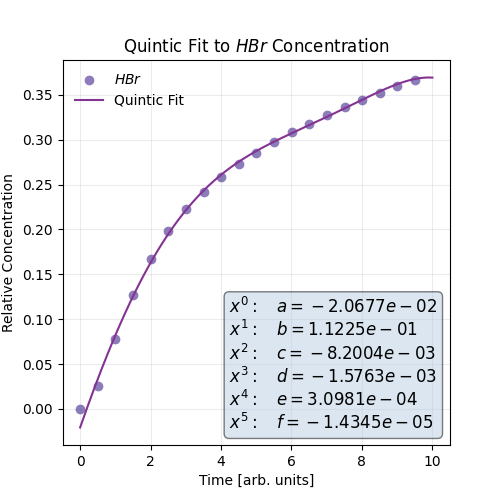
\includegraphics[width=0.6\textwidth]{../HydrogenFusion/Images/quintic-fit.png}
    }
    \caption{Fit polinoma 5. stopnje.}
    \label{fig:br-poly}
\end{figure}

Vidimo da je ujemanje precej dobro. Imel sem željo, da bi določil odvisnost parametrov od začetnih koncentracij,
ampak mi je za to zmanjkalo časa. Imam pripravljen HDF datoteko, kjer so shranjeni vsi podatki, tako da mogoče
nekoč v prihodnosti, ali pa če bo kdo drug imel čas, da se loti tega. Zanimivo se mi je zdelo, da bi kemikom potem 
podal graf hitrosti reakcij v odvisnosti od začetnih koncentracij v vodilnem redu. To pa sem naredil in je 
prikazano na sliki \ref{fig:br-heatmap}, poleg še zahtevanih potekov za različne začetne koncentracije. Narisan je 
tudi primer, ko dodamo ogromno $\mathrm{HBr}$, kjer se vidi, da je reakcija popolnoma nasičena z $\mathrm{HBr}$ in 
se tako nikamor ne premakne. 

\begin{figure}[H]
    \centering
    \makebox[\textwidth][c]{%
    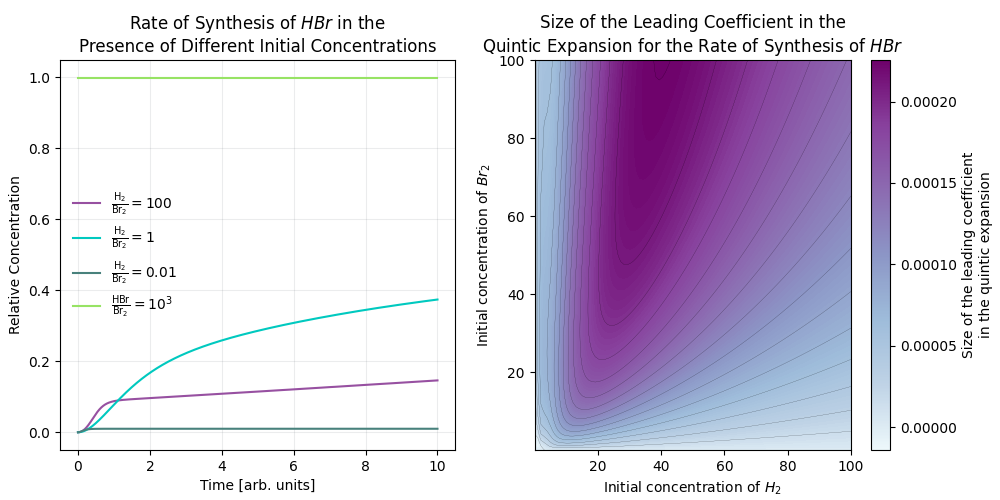
\includegraphics[width=1.2\textwidth]{../HydrogenFusion/Images/rate-plot.png}
    }
    \caption{Hitrost sinteze vodikovega bromida.}
    \label{fig:br-heatmap}
\end{figure}

\subsection{Kemijska ura}
Ta del naloge sem še najbolj na hitro rešil in si želim, da bi si lahko vzel več časa zanj. 
Nisem dejansko prišel do oscilacij, kar bi bilo sicer zelo kul. Vseeno poglejmo prvo primer 
lepe splošne rešitve prikazane na sliki \ref{fig:clock-basic}. 

\begin{figure}[H]
    \centering
    \makebox[\textwidth][c]{%
    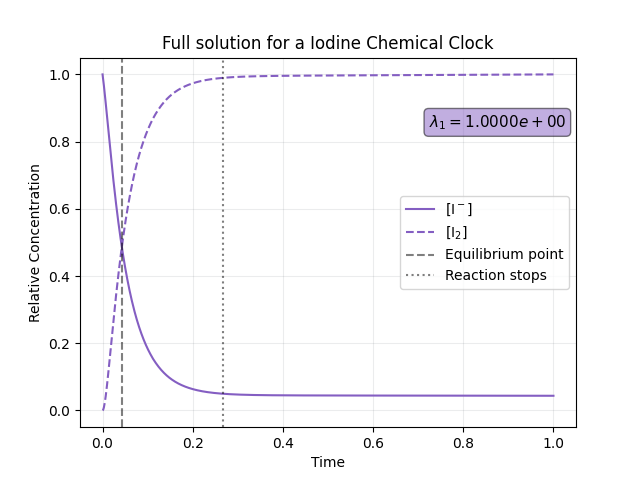
\includegraphics[width=0.8\textwidth]{../ChemicalClock/Images/nice-basic-solution.png}
    }
    \caption{Splošna rešitev kemijske ure.}
    \label{fig:clock-basic}
\end{figure}

Nisem popolnoma prepričan če je to res to kar smo želeli dobiti, ampak koncentraciji Joda in
Jodida se zamenjata torej bi prišlo do spremembe barve. Nisem pa čisto prepričan zakaj potem,
se ne spremeni nazaj. V sistem sem dal dovoljšen presežek tio in persulfata, da bi moralo
priti do tega. Za zahtevana razmerja hitrosti glavnih reakcij sem potem dobil takšno sliko 
\ref{fig:clock-req}.

\begin{figure}[H]
    \centering
    \makebox[\textwidth][c]{%
    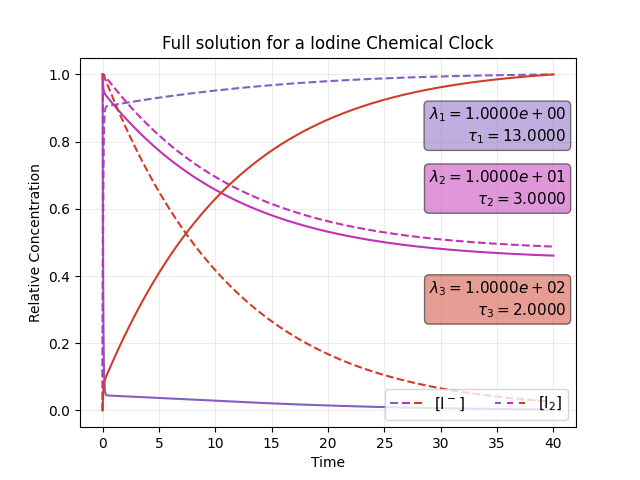
\includegraphics[width=0.8\textwidth]{../ChemicalClock/Images/basic-solutions.png}
    }
    \caption{Rešitev kemijske ure za zahtevana razmerja hitrosti.}
    \label{fig:clock-req}
\end{figure}

Ta graf mi sila ni všeč, ker je obupno nepregleden. Vidi se, da se koncentracija Joda in Jodida
res zamenjata v primeru 1 in 3, ampak v primeru 2 pride pa do neke čudnosti, kjer koncentraciji 
skoraj enako padata. Tako ali tako se primera 1 sploh ne vidi zaradi tako različnih časovnih skal.
Come to think of it, so tudi izmerjeni časi reakcij zelo nenavadni. Nekaj je šlo narobe. A vseeno 
imam še zadnjo sliko kjer sem risal čas potreben, da se reakcija ustavi v odvisnosti od razmerja
hitrosti. To je prikazano na sliki \ref{fig:clock-speed}.

\begin{figure}[H]
    \centering
    \makebox[\textwidth][c]{%
    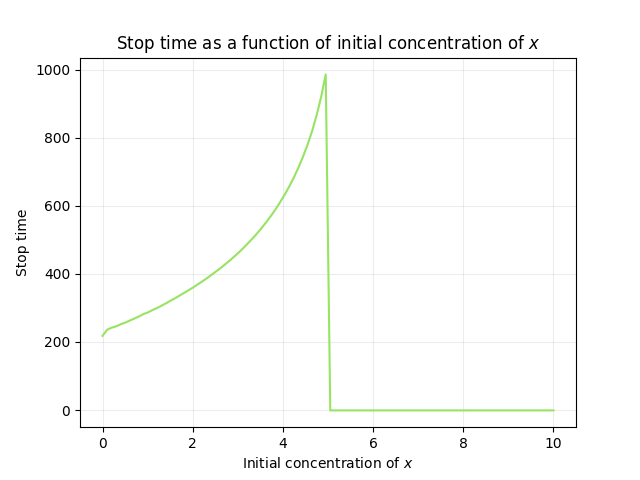
\includegraphics[width=0.8\textwidth]{../ChemicalClock/Images/stop-time.png}
    }
    \caption{Čas potreben, da se reakcija ustavi v odvisnosti $[\mathrm{S}_2\mathrm{O}_3^{2-}](0)$.}
    \label{fig:clock-speed}
\end{figure}

Tu sem imel časovno območje $[0, 1000]$, kar je precej veliko. Pa vidimo da po 5 delih $[\mathrm{S}_2\mathrm{O}_3^{2-}]$
rabi reakcij tako dolgo da se ustavi, da ni več znotraj tega območja. Nisem prepričan zakaj ne gre čas proti $0$ za 
padajočo začetno koncentracijo. To se zdi neka čudna diskrepanca. Ampak tu bom moral zaključiti s poročilom,
ker mi zmanjkuje časa. Ura je 10:14 AM na četrtek.\\


\section{Komentarji in izboljšave}
Želim si, da mi možgan ne bi ta teden delal toliko težav in serviral brezvezne težke vsebine.
To bi mi omogočilo, da bi actually naredil kvalitetno nalogo, ker se mi zdi, da je tole zelo bedna izvedba
in tokrat ni to posledica tega, da bi sam raziskoval neko vzporedno področje. \\

Ampak ne vem če je kaj kar lahko še naredim. Zdravila že jemljem, v terapijo hodim že dolgo. Včasih 
se pač poslabša in je treba to sprejeti. Upam, da se bo kmalu spet izboljšalo. \\

Drugače pa ja, sem imel veliko željo narediti še primer valovanja oksidacije, ki ga je profesor omenil,
ampak ni bilo možno ta teden. 


%\newpage
%\bibliographystyle{unsrt}
%\bibliography{sources}
\end{document}
